\documentclass[12pt]{article}
\usepackage[utf8]{inputenc}
\usepackage[T1]{fontenc}
\usepackage[a4paper,left=2cm,right=2cm,top=2cm,bottom=2cm]{geometry}
\usepackage[french]{babel}
\usepackage[pdftex]{graphicx}
\usepackage{enumitem}
\usepackage{listings}
\usepackage{xcolor}
\usepackage{pdfpages}
\usepackage[a4paper,left=2cm,right=2cm,top=2cm,bottom=2cm]{geometry}
\usepackage{hyperref}
\hypersetup{
	colorlinks=true,
	linkcolor=blue,
	filecolor=magenta,      
	urlcolor=cyan,
	pdftitle={Machine de Turing},
	pdfpagemode=FullScreen,
}

\title{Machine de Turing}
\author{ALLEGRE--COMMINGES Clément et BROUARD Romain}
\date{~}
\begin{document}
	\maketitle
	\tableofcontents
	\section{Introduction}
	\subsection{Un peu d'histoire...}
	En 1928, Le mathématicien allemand David Hilbert énonce le "problème de la décision". Il se demande s'il est possible de trouver une méthode « effectivement calculable » pour décider si une proposition est démontrable. Pour résoudre ce problème, il faut caractériser ce qu'est un procédé effectivement calculable. C'est alors qu'Alan Turing, alors en thèse à Cambridge, conceptualise une machine universelle et prouve grâce à cette dernière que le problème de l'arrêt est indécidable, ce qui permet de donner une réponse négative au problème d'Hilbert pour l'arithmétique. C'est alors qu'Alan Turing introduit les concepts de programme et programmation.\\
	Ce concept de machine universelle, que nous appellerons désormais Machine de Turing Universelle (MTU) n'est pas réalisable puisqu'il s'agit d'un objet mathématique, dont l'on va détailler le fonctionnement plus tard. Néanmoins, une Machine de Turing à état fini peut-être construite, et la première vit donc le jour à Bletchley Park pendand la Seconde Guerre Mondiale, où Turing lui-même et une équipe de scientifique triés sur le volet par le MI6\footnote{Services de renseignement britanniques} construisirent une Machine de Turing pour casser les codes allemands générés par la machine Enigma.\\
	
	\subsection{Fonctionnement d'une MTU}
	Une MTU se compose de deux éléments essentiels :
	\begin{itemize}[label=$-$]
				\item un ruban de taille infinie, divisé en cases.\\
		\item une tête de lecture/écriture (qu'on appellera simplement tête de lecture, même si elle permet également d'écrire sur le ruban)
	\end{itemize}
	Le ruban permet d'accueillir des symboles qui seront lus et écrits par la tête de lecture. Le ruban peut se déplacer vers la gauche ou la droite. L'ensemble des symboles traités est appelé un alphabet.\\
	La tête de lecture permet de lire et écrire un symbole. Elle possède également un état.\\
	\\
	Une machine de Turing marche donc de la manière suivante :\\
	\begin{enumerate}
		\item La tête de lecture lit le symbole qu'elle pointe sur le ruban.\\
		\\ En fonction de son état et du symbole lu, la tête de lecture écrit un symbole à la place de celui qu'elle a lu précédemment.\\
		\item Un déplacement est  choisi en fonction de l'état de la tête de lecture et du symbole lu.\\
		\item La tête de lecture change d'état.\\
		Le ruban se déplace vers la droite ou vers la gauche selon le déplacement choisi précédemment.\\
		\item Puis on recommence depuis le 1.
	\end{enumerate}
	 On peut donc résumer le fonctionnement comme cela : à chaque "cycle", on choisi un symbole à écrire, un nouvel état pour la tête de lecture, et un déplacement, en fonction d'un symbole lu et de l'état actuel. On peut donc définir une fonction de transition, qui va se charger de déterminer l'état futur d'une MTU en fonction de ton état courant. L'ensemble des fonctions de transition permettant de traiter un "mot" peut être représenté sous la forme d'une table de transitions ou d'un graphe de transitions.\\
	 Un mot traité est dit accepté si une Machine de Turing s'arrête en état final après l'avoir intégralement traité.\\
	 Une MTU possède forcément un nombre fini d'états, et elle a au moins deux états obligatoires : $q_O$ l'état initial, et $F$ un ensemble d'états d'acceptation.\\
	 \\
	 Une machine de Turing est donc définie par :\\
	 \begin{itemize}[label=$-$]
	 	\item $Q$ un ensemble fini d'états.\\
	 	\item $q_0$ un état initial tel que $q_0 \in Q$.\\
	 	\item $F$ un ensemble d'états d'acceptation tel que $F \subseteq Q$.\\
	 	\item $\Gamma$ un ensemble fini de symboles.\\
	 	\item $\Sigma$ un ensemble fini de symboles d'entrée tel que $\Sigma \subseteq \Gamma$.\\
	 	\item $B$ un symbole de ruban vide tel que $B \in \Gamma \setminus \Sigma$.
	 	\item $\delta$ une fonction de transition.
	\end{itemize}
	 Une fonction de transition se formalise donc comme ceci :\\
	 \[ \delta (q, Z) \to (p, Y, D) \]
	 avec $q$ l'état de la tête de lecture, $Z$ le symbole pointé, $p$ le nouvel état, $Y$ le nouveau symbole et $D$ le déplacement.\\
	 \\
	 Exemple d'une table de transition pour une Machine de Turing acceptant le langage $L = \lbrace a^kb^k \, \vert \, k > 0 \rbrace$ avec $q_0$ comme état initial (représenté par une $\to$), et $q_4$ comme état d'acceptation (représenté par $\ast$):\\
	 \\
	 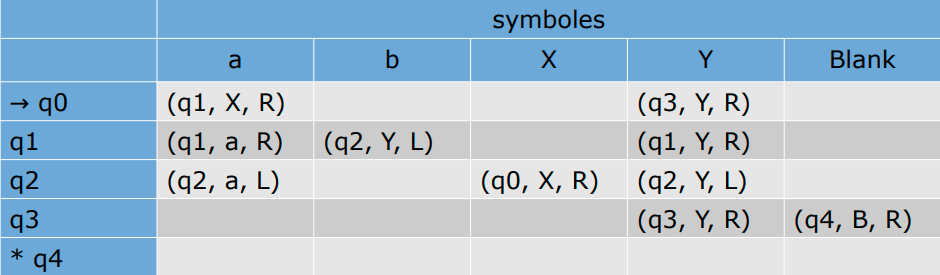
\includegraphics[width=\textwidth]{img/fig1}
	 \\
	 Le but de ce projet va donc être de concevoir une Machine de Turing telle que définie ci-dessus.
	 \section{Conception}
	 \subsection{Cahier des charges}
	 Le cahier des charges est composé de trois parties. La partie 1 doit être traitée absolument, les parties 2 et 3 seront traitées si le temps nous le permet.
	 \subsubsection{Partie 1}
	 Dans un premier temps, le système conçu doit être capable de :\\
	 \begin{itemize}[label=$-$]
	 	\item exécuter un programme prédéfini (codé en dur dans le programme microcontrôleur).\\
	 	\item avoir un mode pas à pas pour l'exécution du programme.\\
	 	\item avoir un mode continu pour l'exécution du programme.\\
	 	\item gérer l'affichage de l'état du ruban.\\
	 	\item gérer l'affichage de la position de la tête de lecture.\\
	 	\item gérer l'affichage de la table de transition.
	 \end{itemize}
	 \subsubsection{Partie 2}
	 Dans un second temps, il faut rajouter :\\
	 \begin{itemize}[label=$-$]
	 	\item  la possibilité de sélectionner un programme via un menu.\\
	 	\item le stockage des programmes à sélectionner.\\
	 	\item l'initialisation manuelle du ruban et de la position de la tête de lecture.
	 \end{itemize}
	 \subsubsection{Partie 3}
	 Enfin pour obtenir un système complet, il faut implémenter :\\
	 \begin{itemize}[label=$-$]
	 	\item la programmation directement sur la machine d'une table de transition.\\
	 	\item l'enregistrement de la table de transition programmée dans le support de stockage.\\
	 	\item un reset de la programmation de la ligne en cours.\\
	 	\item l'affichage d'une description du programme.
	 	\end{itemize}
	 \subsection{Conception Matérielle}
	 Pour concevoir notre système, nous avons décidé de traiter les trois parties en même temps, ce qui nous évite de devoir repasser par une phase de conception et d'adaptation lors de la réalisation des parties 2 et 3.\\
	 \subsubsection{SFN1}
	 Nous avons donc commencé par dessiner un Schéma fonctionnel de premier niveau, pour définir les différentes entrées et sorties de notre système :\\
	 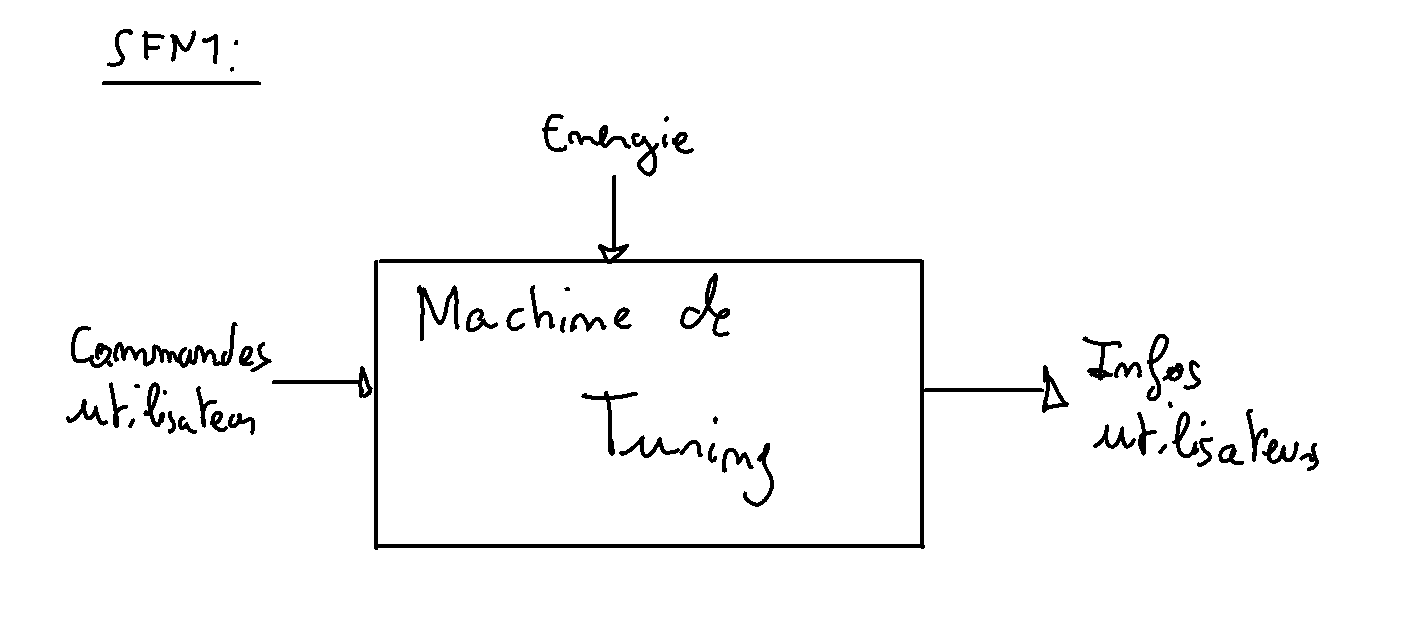
\includegraphics[width=\textwidth]{img/SFN1}
	\subsubsection{SFnD}
	On peut désormais rentrer un peu plus dans le détail avec un SF1D :\\
	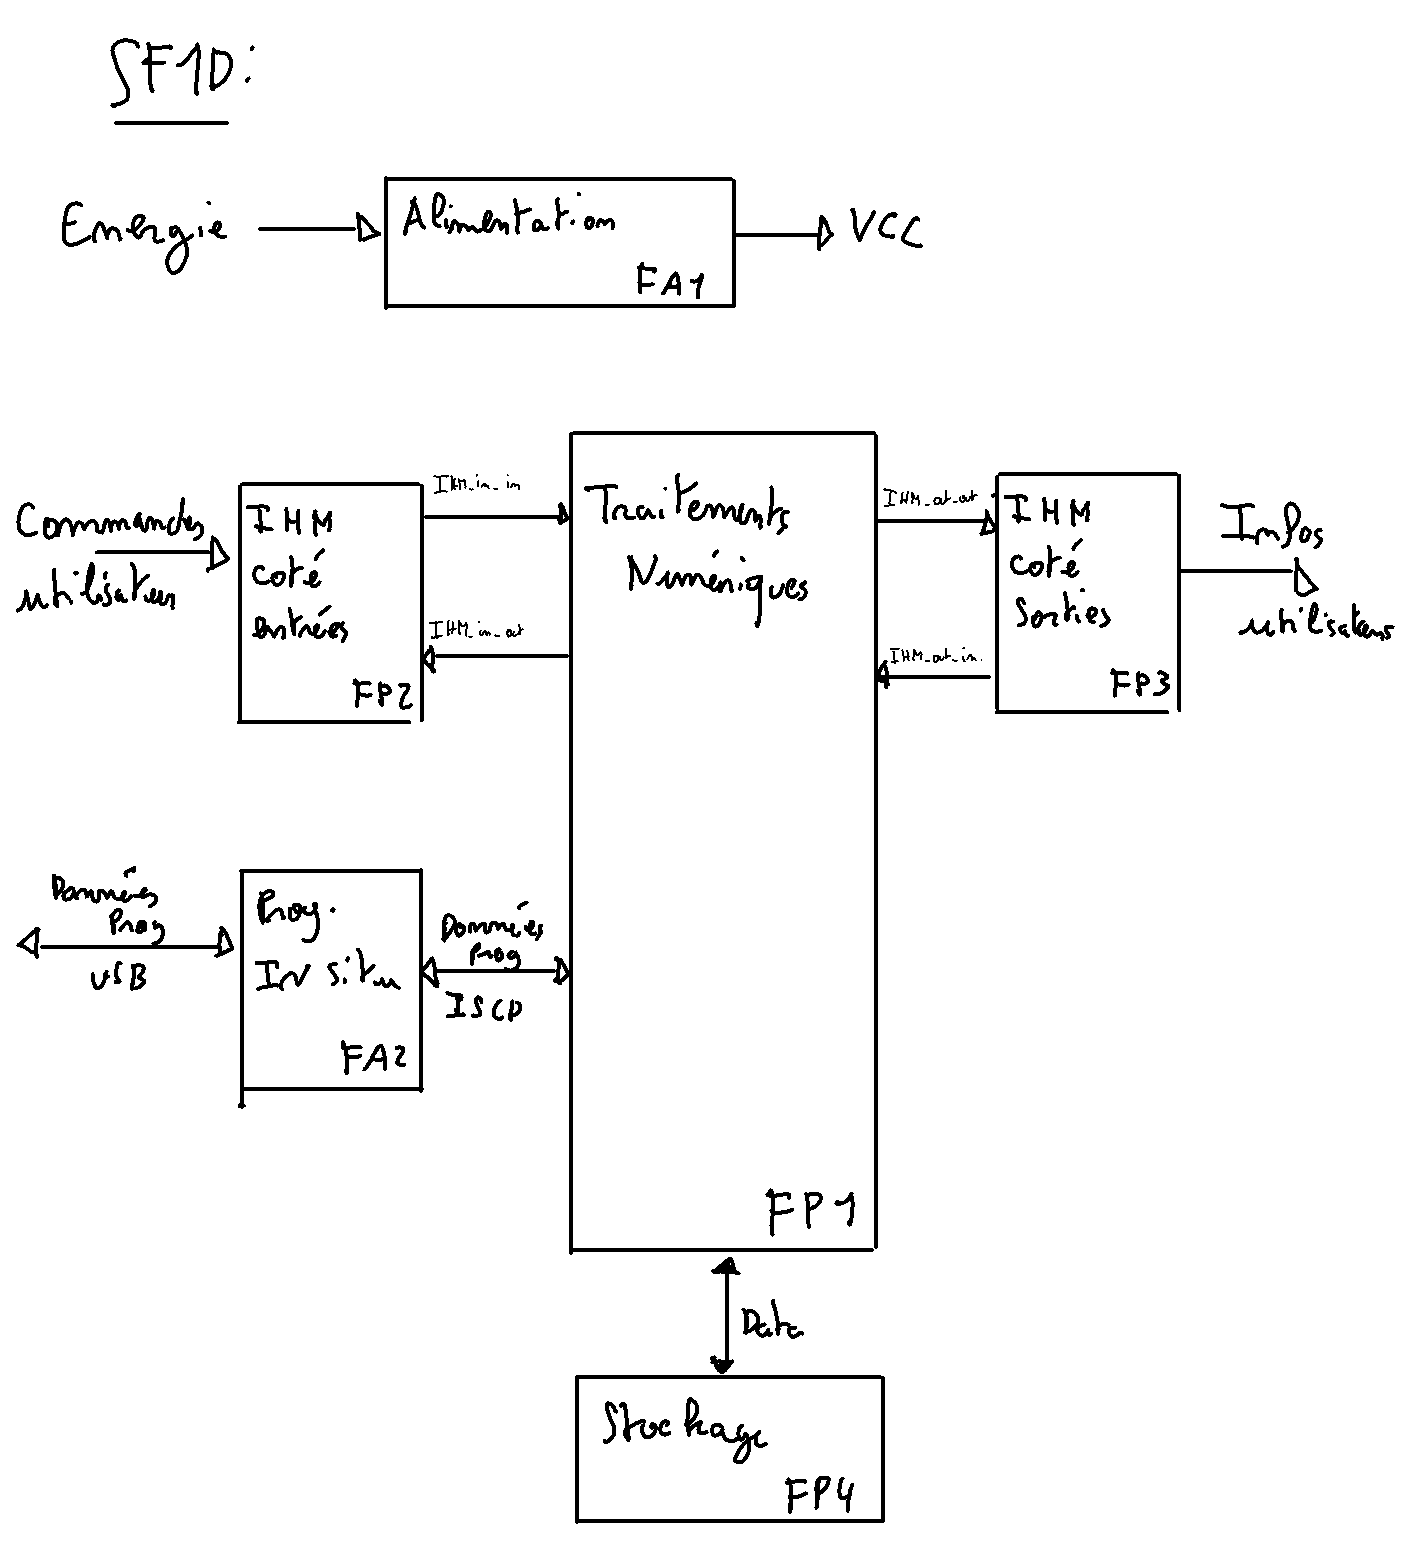
\includegraphics[width=\textwidth]{img/SF1D}
	On voit qu'on a quatre fonctions principales : une qui s'occupe de la gestion des entrées (FP2), une qui gère les sorties (FP3), une fonction de stockage pour stocker les tables de transitions (FP4), et du traitement numérique qui va piloter tout ça (FP1).\\
	On a aussi deux fonctions annexes : la fonction alimentation qui va se charger de fournir le courant nécessaire pour que la machine puisse fonctionner, et la fonction de programmation in-situ qui va faciliter le chargement du code dans la machine et nous éviter d'avoir à sortir le micro-contrôleur (MCU) à chaque fois.\\
	\\
	On voit que les fonctions FP2 et FP3 sont encore floues, on va donc les affiner en faisant des SF2D pour qu'on se rende compte de leur fonctionnement :\\
	\paragraph{FP2 :}
	\includegraphics[width=\textwidth]{img/SF2DFP2}
	On voit clairement que FP2 est bien plus complexe qu'elle ne le parait, et forme un ensemble de fonctions plus spécifiques qui vont permettre à l'utilisateur d'interagir physiquement avec la machine, dans le but de la configurer, programmer, etc.
	\paragraph{FP3 :}
	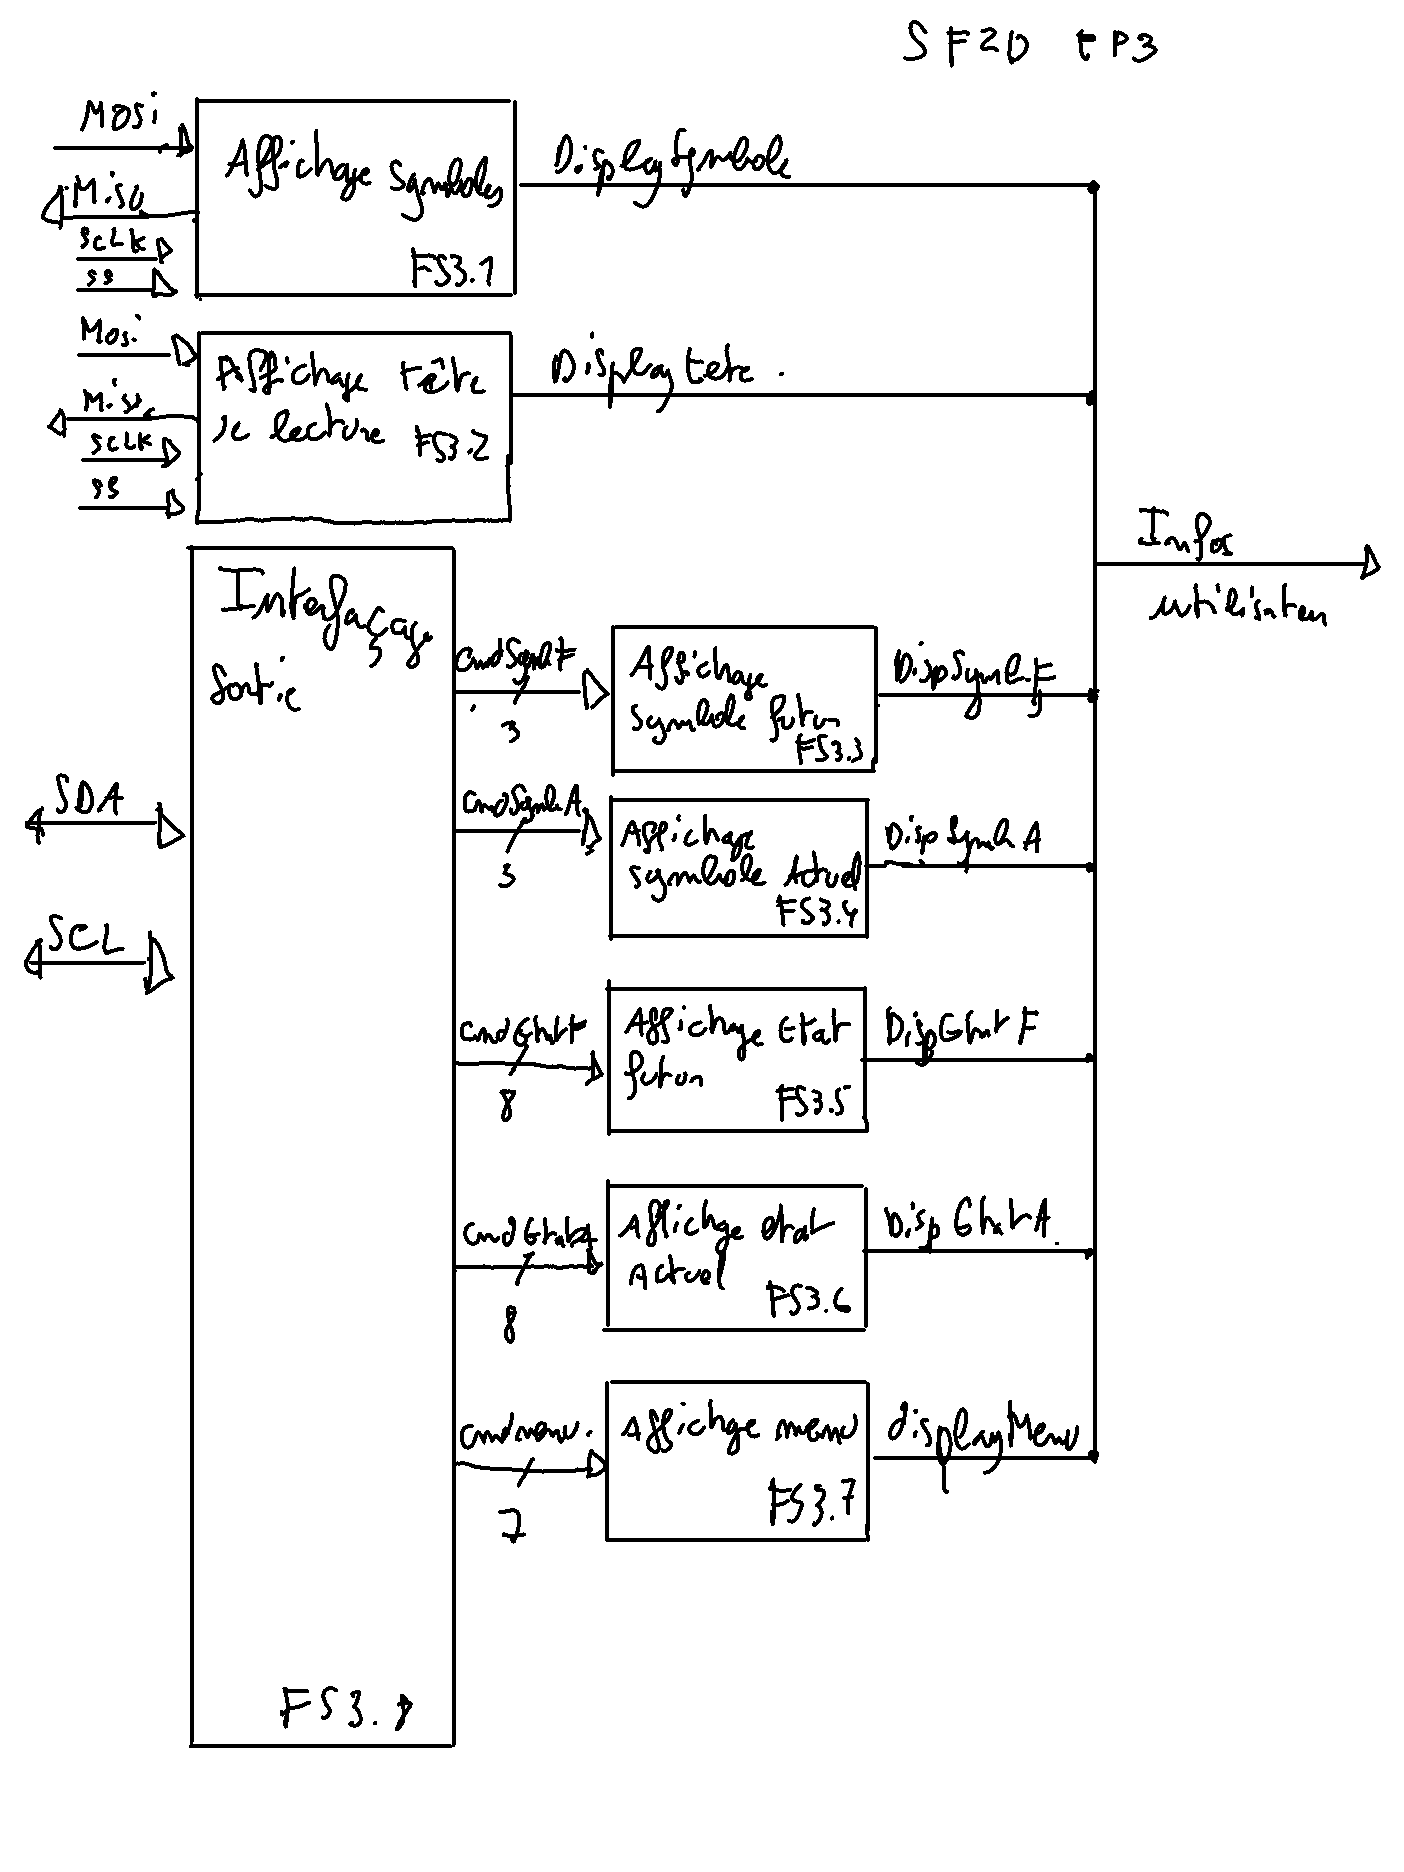
\includegraphics[width=\textwidth]{img/SF2DFP3}
	De la même manière que pour FP2, FP3 est en réalité un ensemble de fonctions plus spécifiques qui vont chacune avoir un rôle bien précis dans le retour des informations utilisateur. On a donc une grande variété de fonctions d'affichage qui vont, de la même manière que pour les sous-fonctions de FP2, être spécifiées ci-dessous.
	\subsubsection{Spécifications des fonctions et de leurs signaux de communication}
	Nous avons donc spécifié ci-dessous, pour chaque fonction, son rôle ainsi que ses signaux d'entrée et/ou de sortie. Nous avons également précisé le rôle ainsi que ce qui fait l'essence même de chaque signal (type, etc.).
	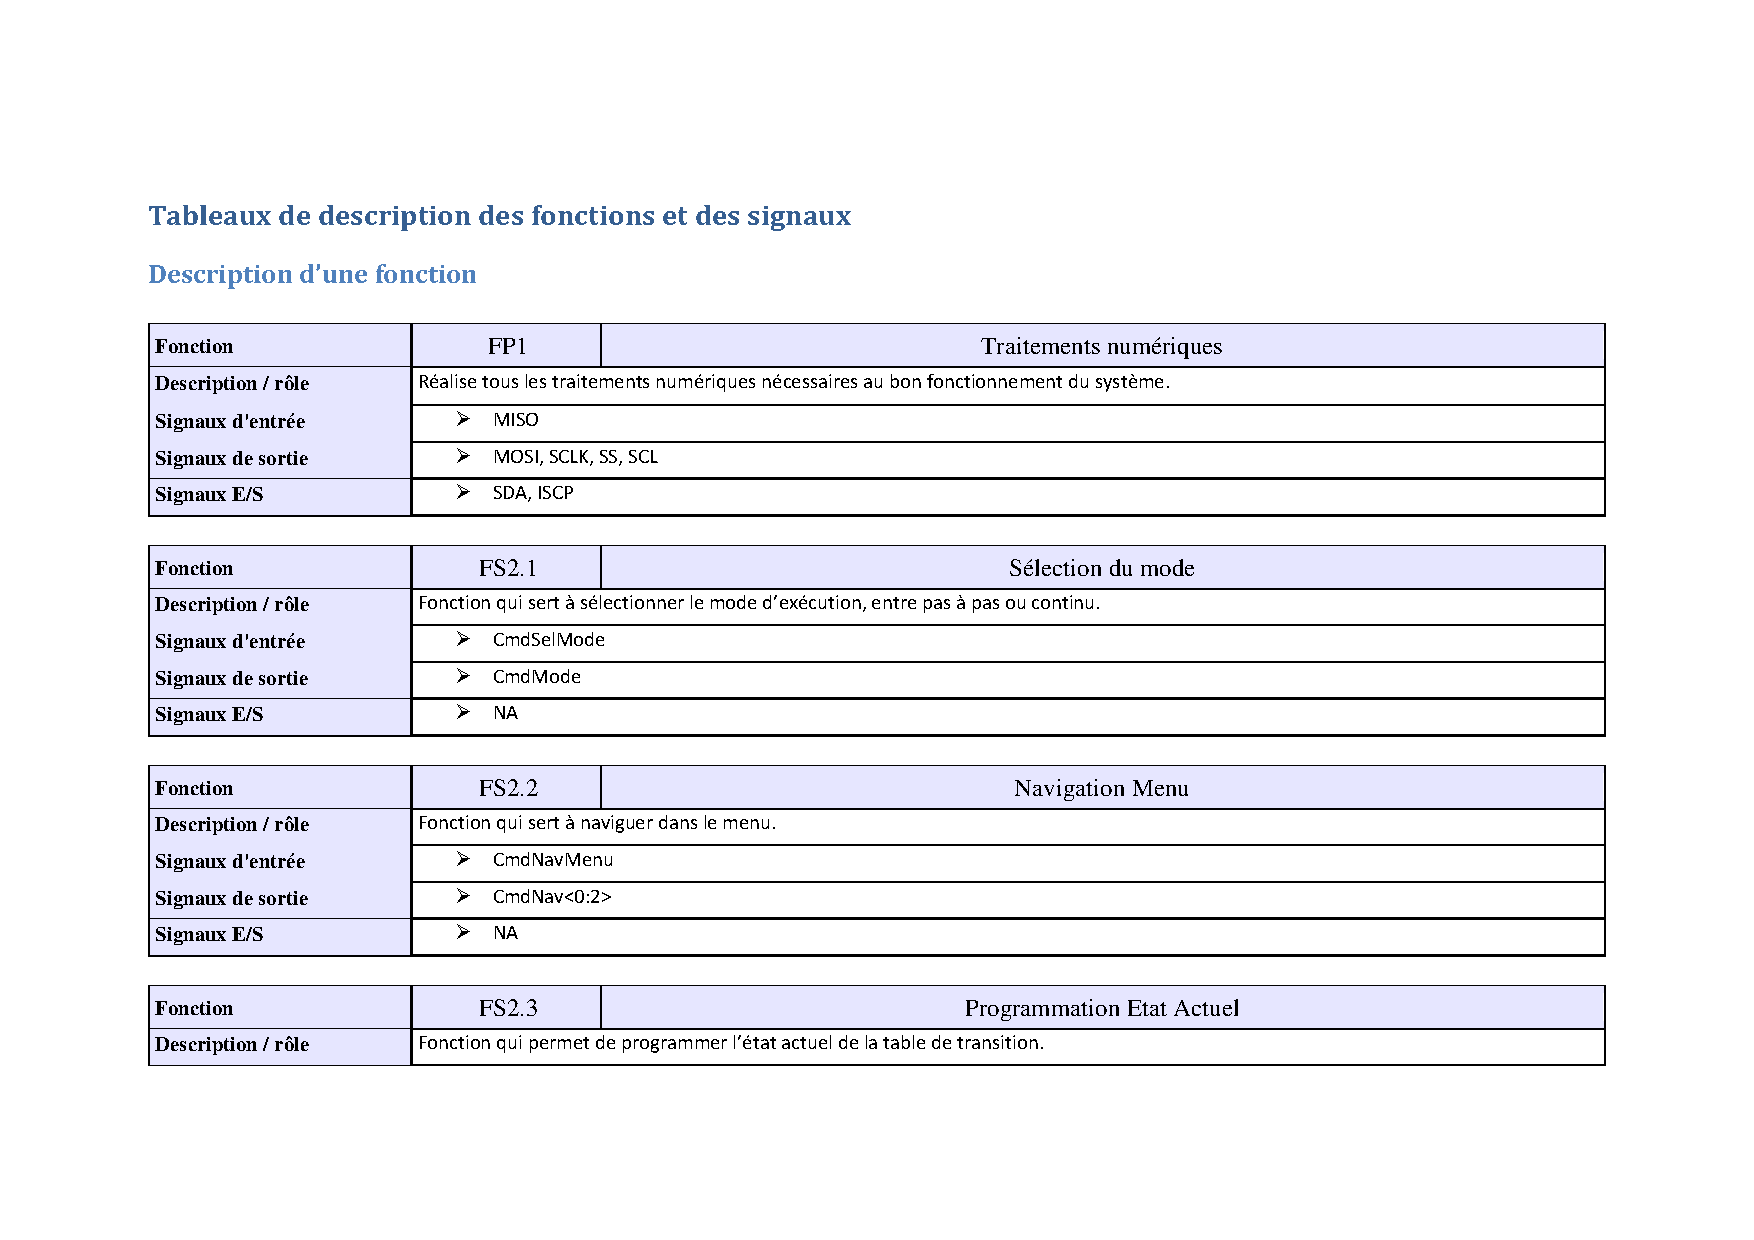
\includepdf[pages=-]{docs/specs_fonctions_signaux}
	\subsubsection{Choix des composants}
	Nous pouvons désormais choisir nos composants. Nous avons donc choisis les références suivantes :
	\begin{itemize}[label=$-$]
		\item rubans de leds adressables $\times$ 2 : \url{https://www.superlightingled.com/sk9822similar-to-apa102-digital-intelligent-dream-color-rgb-72ledsm-dc5v-addressable-led-strip-lights-p-3256.html}
		\item afficheurs 7 segments $\times$ 2 : \url{https://fr.farnell.com/broadcom-limited/hdsm-283b/afficheur-a-led-cms-7mm-bleu-cc/dp/1659312}
		\item leds adressables RGB $\times$ 2 : \url{https://www.gotronic.fr/art-led-rgb-5-mm-rgb5-dif-2099.htm} (à interfacer)
		\item expendeurs IO - I²C $\times$ 2 : \url{https://www.mouser.fr/ProductDetail/Texas-Instruments/TCA6424ARGJR?qs=Ze4%2FuFuz19LzqLgNFpYqlQ%3D%3D}
		\item écran LCD $\times$ 1 : TSB1G7000-E
		\item boutons poussoirs $\times$ 2 : A voir avec Sébastien Beaufils
		\item commutateurs $\times$ 2 : idem
	\end{itemize}
	\subsubsection{Schéma représentatif et schéma électrique}
	\subsubsection{Tests}
	\subsection{Conception Logicielle}
	
	\section{Annexes}
	\subsection{Sources}
\end{document}